\problem{Image Restoration}
(a) The spectrum of the origin image is generated through FFT.\\
To shift the zero frequency to the center of the spectrum, we times $(-1)^{u+v}$ for each pixel $(u,v)$ on the origin image before applying FFT.

To have a better effect of visualization on the frequency domain, the image is shown by applying the log transformation on the magnitude of the Fourier transform of the image.\\
i.e. $I_{\text{log}}=20\log(1+|I|)$, where $I$ is the spectrum generated by Fourier transform of the image.

\begin{figure}[htbp]
    \centering
	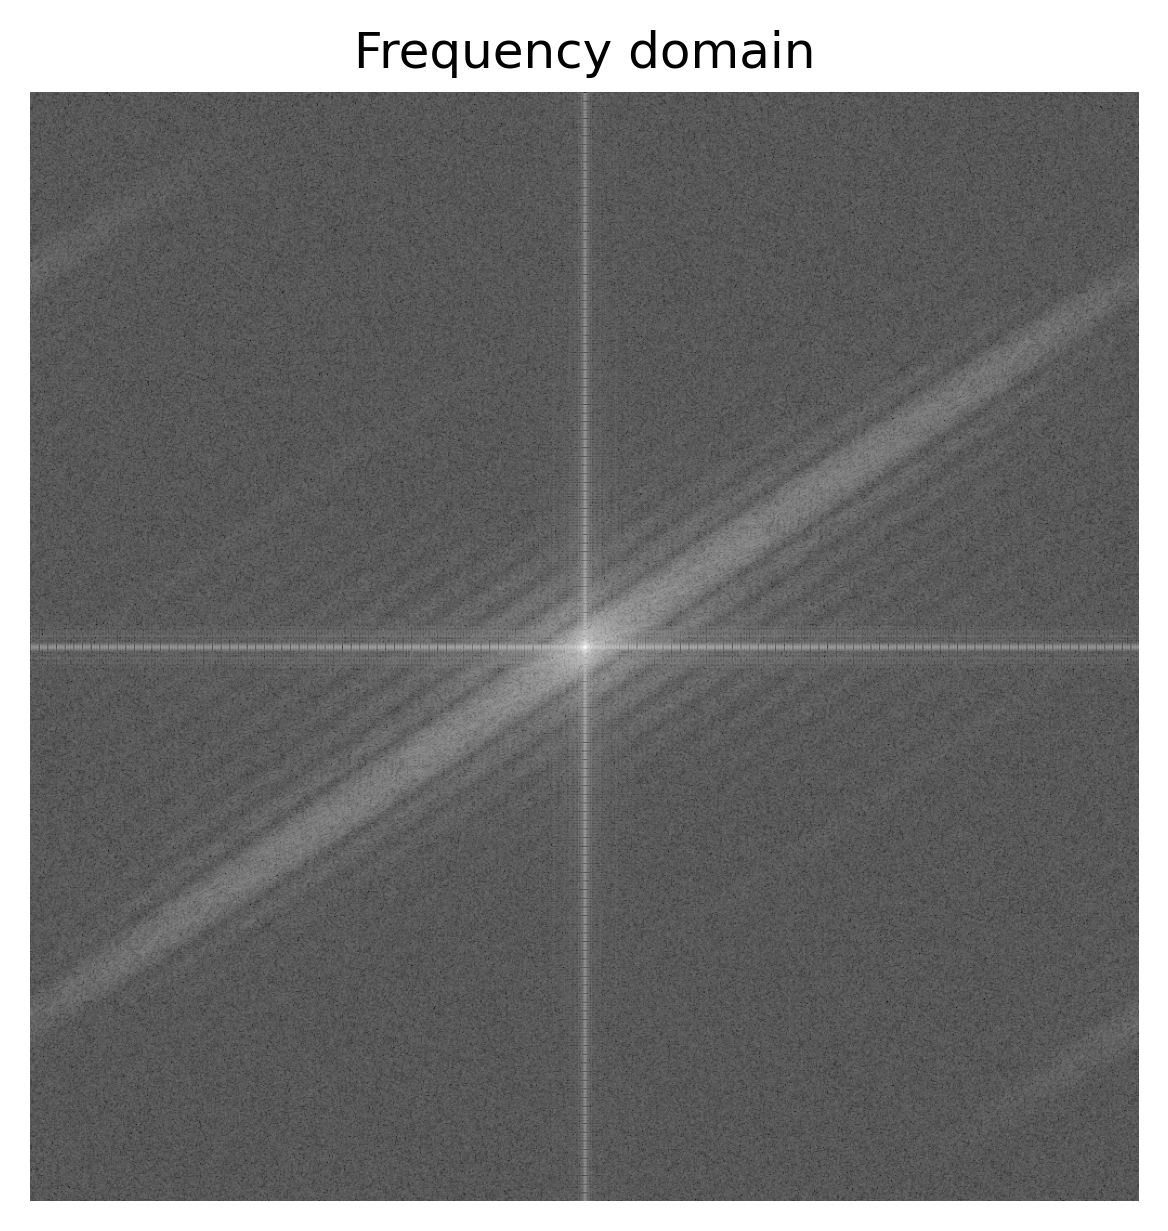
\includegraphics[width=0.5\textwidth]{../images/p4/p4a.png}
    \caption{FFT shifted spectrum}
    \label{fig:p4a}
\end{figure}

(b) The image by applying Radon transform on the origin image is shown in Figure \ref{fig:p4b}.\\
We can get the coordinates with the highest intensity in the Radon transformed image, which is $(\theta,d)=(,)$.\\

So above all, the angle between the strip and the vertical direction is $\theta=$
and the distance between two similar dark strips is $d=$

$N=640,L=\dfrac{N}{d}=$

% \begin{figure}[htbp]
%     \centering
% 	\includegraphics[width=\textwidth]{../images/p4/p4b.png}
%     \caption{Radon Transformed image}
%     \label{fig:p4b}
% \end{figure}




(c)


% \begin{figure}[htbp]
%     \centering
% 	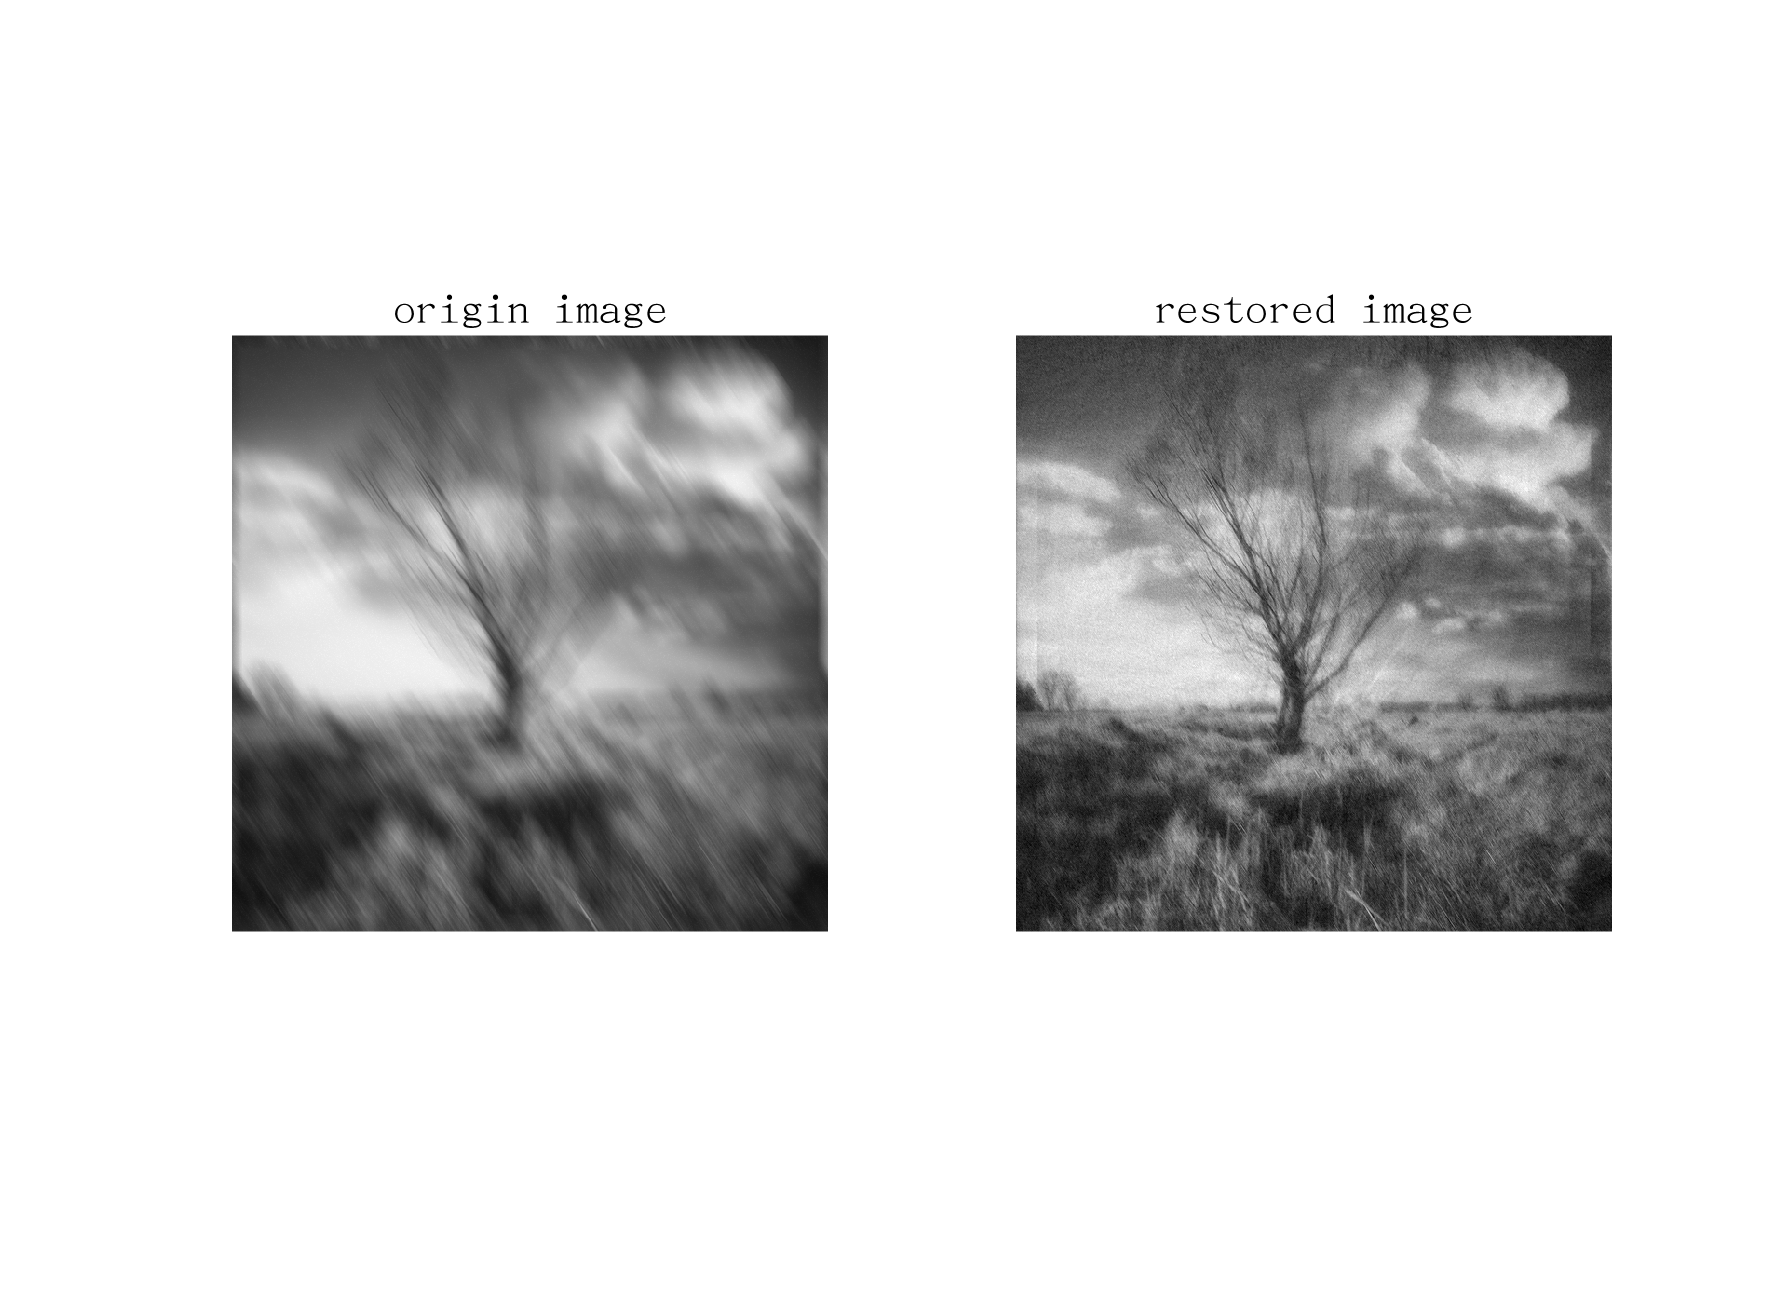
\includegraphics[width=\textwidth]{../images/p4/p4c.png}
%     \caption{p4c}
%     \label{fig:p4c}
% \end{figure}





\newpage